\documentclass[a4paper,11pt]{article}
%\usepackage[T1]{fontenc}

%\setlength{\textwidth}{20cm}
%\setlength{\marginparwidth}{0cm}
%\setlength{\voffset}{0cm}
\usepackage[utf8]{inputenc}
\usepackage[francais]{babel}
\usepackage{amsmath}
\usepackage{graphicx}


\usepackage[dvipsnames]{xcolor}
\definecolor{beaublue}{rgb}{0.74, 0.83, 0.9}
\definecolor{aliceblue}{rgb}{0.94, 0.97, 1.0}
\usepackage[framemethod=default]{mdframed}
\newmdenv[linecolor=black,backgroundcolor=aliceblue]{cadre}

%\special{papersize=210mm,297mm}
\title{{\Huge Electronique numérique}\\Logique combinatoire}
%\title{TD1}
\date{}

\begin{document}
\maketitle
{\bf Remarque} : tous les exercices ne seront pas forcément traités en TD.

%==========================================================================
\section{Equations logiques de circuits de base}

\subsection{Additionneur}
\begin{enumerate}
\item Etablir la table de vérité d'un {\it demi-additionneur} logique, puis les deux équations logiques associées : ce circuit additionne simplement 2 entrées booléennes $a$ et $b$
(donc {\it sans retenue entrante}). Il calcule deux sorties : la somme et la retenue sortante. Dessiner le circuit.

\begin{cadre}
  {\bf Solution}\\

  \begin{tabular}{|c|c||c|c|}
    \hline
    a & b & s & $c_o$  \\
    \hline
    0 & 0 & 0 & 0 \\ \hline
    0 & 1 & 1 & 0 \\ \hline
    1 & 0 & 1 & 0 \\ \hline
    1 & 1 & 0 & 1  \\ \hline
  \end{tabular}
  On trouve :
  $
  \begin{cases}
    s = a \oplus b \\
    c_o = a.b \\
    \end{cases}
  $

\end{cadre}


\begin{figure}[!h]
  \centering
  \fbox{\includegraphics[scale=0.4]{ha.png}}
  \caption{Circuit ('netlist') du demi-additionneur 1 bit}
  \label{ha}
\end{figure}

\item Etablir la table de vérité d'un {\it additionneur complet} pour deux opérandes 1 bit. Ce dernier tient désormais compte d'une retenue entrante. Etablir les équations simplifiées des sorties, puis dessiner le circuit correspondant. Au préalable on démontrera que :
$$\overline{x\oplus y}=x \oplus \overline{y}$$

\begin{cadre}
{\bf Solution}\\
On écrit la table de vérité, comme précédemment :\\
\begin{tabular}{|c|c|c||c|c|}
  \hline
  a & b & $c_i$ & s & $c_o$  \\ \hline
  0 & 0 & 0 & 0 & 0 \\ \hline
  0 & 0 & 1 & 1 & 0 \\ \hline
  0 & 1 & 0 & 1 & 0 \\ \hline
  0 & 1 & 1 & 0 & 1 \\ \hline
  1 & 0 & 0 & 1 & 0 \\ \hline
  1 & 0 & 1 & 0 & 1 \\ \hline
  1 & 1 & 0 & 0 & 1 \\ \hline
  1 & 1 & 1 & 1 & 1 \\ \hline
\end{tabular}
On trouve :

\begin{align*}
  s &= \overline{a} . \overline{b} . c_i  +  \overline{a} . b . \overline{c_i}  +  a . \overline{b} . \overline{c_i}  +  a . b . c_i \\
  c_o &= \overline{a} . b . c_i  +  a . \overline{b} . c_i  +  a . b  +  \overline{c_i}  +  a . b . c_i \\
\end{align*}

On peut simplifier ces deux équations :

\begin{align*}
  s &= \overline{a}.(b \oplus c_i) + a.(b \oplus \overline{c_i}) \\
  c_o &= a.b+c_i.(a \oplus b)\\
\end{align*}

La première équation (la somme) peut s'écrire autrement, ce qui nous permettra de reconnaître les équations du demi-additionneur.
Pour cela on démontre que $\overline{x \oplus y} = x \oplus \overline{y}$. On a :
\begin{eqnarray}
\overline{x \oplus y}  & = & \overline{x.\overline{y}+\overline{x}.y} \nonumber \\
                       & = & \overline{x.\overline{y}}.\overline{\overline{x}.y} \nonumber \\
                       & = & (\overline{x}+y).(x+\overline{y}) \nonumber \\
                       & = & \overline{x}.x+\overline{x}.\overline{y}+x.y+y.\overline{y} \nonumber \\
                       & = & 0 + \overline{x}.\overline{y}+x.y + 0\nonumber \\
                       & = & x \oplus \overline{y} \nonumber
\end{eqnarray}

On pose $ \alpha = b \oplus c_i$ . On trouve que :
\begin{align*}
  s &= \overline{a}.(b \oplus c_i) + a.(b \oplus \overline{c_i}) \\
    &= \overline{a}.\alpha + a .\overline{\alpha} \\
    &= \overline{a} \oplus \alpha \\
    &= a \oplus b \oplus c_i
\end{align*}

En résumé :
    \begin{align*}
      s   &= a \oplus b \oplus c_i \\
      c_o &= a.b+c_i.(a \oplus b)
    \end{align*}

\end{cadre}

\item Montrer qu'un additionneur complet ``1 bit'' peut réutiliser le demi-additionneur de la question 1.

\begin{figure}[!h]
  \centering
  \fbox{\includegraphics[scale=0.3]{full_adder.png}}
  \fbox{\includegraphics[scale=0.4]{full_adder_ha.png}}
  \caption{Circuit ('netlist') de l'additionneur 1 bit complet (full-adder 1 bit)}
  \label{ha}
\end{figure}

\item Dessiner un additionneur 4 bits en réutilisant l'additionneur 1 bit.
\begin{cadre}
  On propose ci-dessous 2 solutions : la première ne permet pas l'utilisation de retenue entrante, tandis que la seconde
  utilise une telle retenue. Dans le premier cas, il n'est alors pas nécessaire de recourir à un full adder. La seconde
  solution est parfaitement régulière en terme d'aboutement, constituée de full-adder 1 bit.
\end{cadre}

\begin{figure}[!h]
  \centering
  \fbox{\includegraphics[scale=0.25]{adder_4_wo_carry.png}}
  \caption{Additionneur 4 bits sans retenue entrante}
  \label{fa}
\end{figure}

\begin{figure}[!h]
  \centering
  \fbox{\includegraphics[scale=0.3]{adder_4.png}}
  \caption{Additionneur 4 bits avec retenue entrante}
  \label{fa}
\end{figure}

\item Quel est le chemin critique de ce dernier circuit ? On rappelle que le chemin critique est le parcours le plus long entre une entrée et une sortie combinatoire. On le mesurera en nombre de portes logiques élémentaires traversées.
\end{enumerate}

\begin{cadre}
  Il est précisé dans l'exercice que le chemin critique peut être mesuré en nombre de portes ``abstraites'' traversées, donc sans unité physique. Dans la réalité, chacune des portes logiques sera pré-caractérisée par des temps de traversée donnés par le constructeur (Intel, IBM, TSMC.,..) et il faudra donc sommer des {\it temps}. L'exercice vous simplifie un peu la vie : des outils d'{\it analyse de timing} permettent d'automatiser cette tâche fastidieuse. Les {\it synthétiseurs logiques} contiennent également un tel algorithme.\\

Nommons les étages de 0 à 3. Nous devons gérer deux cas distincts correspondants aux 2 solutions précédentes : avec ou sans retenue entrante.
  \begin{enumerate}
    \item Sans retenue entrante : dans ce cas, l'additionneur de l'étage 0 a un chemin critique à partir des entrées. Ce chemin traverse 2 demi-additionneurs, suivi d'un OU logique. Ce qui fait un total de 3 portes logiques. Les autres étages de 1 à 3 ont un chemin critique qui se situe entre l'entrée $C_{in}$ et $C_{cout}$, soit 1 demi-additionneur , suivi d'un OU, ce qui fait, pour chacun des étages, un chemin critique de 2. Pour les 3 étages cela donne donc 6 portes traversées. Le résultat est donc {\bf $3+6=9$} portes pour l'ensemble.
   \item Avec retenue entrante : le même raisonnement conduit à {\it bf 7 portes traversées}, sur le chemin critique.  
  \end{enumerate}

{\bf remarque:} si on place un $0$ (définitif) en entrée du premier cas traité, le chemin réel traversé sera $7$. Par contre, structurellement, c'est 9 portes qui existent. Ces 9 portes constituent un ``faux chemin combinatoire critique''.
\end{cadre}

\subsection{Multiplexeur}
La fonction (combinatoire) d'un multiplexeur est de sélectionner, grâce à un signal de contrôle, un signal d'entrée parmi plusieurs et de transmettre sa valeur sur une sortie unique.
\begin{enumerate}
\item Dessiner le symbole communément admis pour représenter un multiplexeur à 2 entrées binaires (chacune codée sur un 1 bit).
\item Calculer l'équation d'un multiplexeur à 2 entrées 1 bit.
%\item On pourrait de même calculer l'équation d'un multiplexeur à $3,4,\dots$ entrées, sur un 1 bit. Sans recourir à un tel calcul, dessiner la structure d'un multiplexeur à 3 entrées, à base de multiplexeurs à 2 entrées.
\item Lorsque les données d'entrées sont codées sur $n>1$ bits, chacun des bits du signal multiplexé suit évidemment un chemin similaire. Dessiner un tel multiplexeur à 2 entrées, pour $n=2$.
\end{enumerate}

\begin{cadre}
Solution : on parle de multiplexeur 2-vers-1 pour se référer au nombre de voies en entrées. La solution est donnée sur le schéma \ref{mux}.
\end{cadre}

\begin{figure}[!h]
  \centering
  \fbox{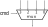
\includegraphics[scale=0.25]{mux.png}}
  \caption{Multiplexeur 2 vers 1, codé sur 1 bit : symbole commun et circuit}
  \label{mux}
\end{figure}

\section{Formes canoniques}

Toute fonction booléenne $F$ de plusieurs variables peut s'écrire sous deux formes spéciales, appelées {\it formes canoniques} : il ne s'agit ni plus ni moins que de l'expression de $F$ sous forme de :
\begin{itemize}
\item ({\bf première forme}) : somme de produits de chaque variable {\it ou de son complément}
\item ({\bf seconde forme}) : produit de sommes de chaque variable {\it ou de son complément}
\end{itemize}

Pour obtenir la première forme à partir de leur table de vérité, il suffit de sommer les produits pour lesquels la fonction vaut '1'. La seconde forme s'obtient de manière duale. Notons que ces formes ne sont pas simplifiées.

Etablir les deux formes canoniques des fonctions suivantes:

\begin{enumerate}
\item $F_1=xy+yz+xz$
\item $F_2=x+yz+\overline{y}.\overline{z}.t$
\end{enumerate}

  {\bf solutions }

  \begin{figure}[!h]
  \begin{center}
  \includegraphics[scale=0.8]{./te1-douillar-1.png}
  \end{center}
  \end{figure}

  \begin{figure}[!h]
  \begin{center}
  \includegraphics[scale=0.5]{./te1-douillar-2.png}
  \end{center}
  \end{figure}

\newpage

\section{Quelques formulations booléennes}

Ecrire sous la première forme canonique les fonctions définies par les propositions suivantes :

\begin{enumerate}
\item $F(a,b,c)=1$ si et seulement si aucune des variables $a,b,c$ ne prend la valeur 1.
\item $F(a,b,c)=1$ si et seulement si au plus une des variables $a,b,c$ prend la valeur 0.
\end{enumerate}

%\begin{cadre}
  {\bf solutions}
  \begin{figure}[h]
  \begin{center}
  \includegraphics[scale=0.5]{./te1-douillar-3.png}
  \end{center}
  \end{figure}
%\end{cadre}

\section{Simplifications algébriques}
Simplifier algébriquement les  fonctions suivantes

\begin{enumerate}
\item $F=\overline{x}.\overline{y} + xy+\overline{x}y$
\item $F=(x+\overline{y})(x\overline{y}+z)z$
\end{enumerate}

\begin{cadre}
  {\bf solutions}
  \begin{enumerate}
  \item $F=\overline{x} + y$
  \item $F=(x+\overline{y}).z$
  \end{enumerate}
\end{cadre}

\section{Simplifications par tableaux de Karnaugh}
Simplifier, par la méthode des tableaux de Karnaugh, les fonctions booléennes suivantes. Dessiner le circuit correspondant et déterminer son chemin critique, en supposant que toutes les portes présentent un temps de propagation de 5 ns. Tous les problèmes ne seront pas forcément résolus en TE.

\subsection{K-map à 3 variables}
\begin{enumerate}
\item $F(a,b,c)=\overline{a}\overline{b}c+\overline{a}b\overline{c}+ab\overline{c}$
\item $F(a,b,c)=\overline{a}b\overline{c}+\overline{a}bc+ab\overline{c}$
\item $F(a,b,c)=\overline{a}\overline{b}c+a\overline{b}\overline{c}+ab\overline{c}$, sachant que la valeur de $F$ pour les combinaisons $\overline{a}bc$ et $abc$ est indifférente.
\end{enumerate}
\begin{cadre}

{\bf solutions}
  \begin{enumerate}
  \item $F(a,b,c)=\overline{a}\overline{b}c+b\overline{c}$
  \item $F(a,b,c)=\overline{a}b+b\overline{c}$
  \item $F(a,b,c)=\overline{a}c+a\overline{c}=a\oplus c$
  \end{enumerate}
\end{cadre}

\subsection{K-map à 4 variables}

$F(a,b,c,d)=\overline{a}b\overline{c}\overline{d} +
            \overline{a}b\overline{c}d+
            \overline{a}bcd+
            \overline{a}bc\overline{d}$

$F(a,b,c,d)=\overline{a}\overline{b}\overline{c}d +
            \overline{a}\overline{b}cd +
            a\overline{b}\overline{c}d +
            a\overline{b}cd$
\begin{cadre}
{\bf solutions}
$$F(a,b,c,d)=\overline{a}b$$
$$F(a,b,c,d)=\overline{b}d$$
\end{cadre}
\subsection{K-map à 5 variables}

$F(a,b,c,d,e)=\overline{a}\overline{b}\overline{c}\overline{d}\overline{e} +
              \overline{a}\overline{b}c\overline{d}\overline{e} +
              \overline{a}b\overline{c}\overline{d}\overline{e} +
              \overline{a}bc\overline{d}\overline{e} +
              ab\overline{c}\overline{d}\overline{e} +
              ab\overline{c}d\overline{e} +
              abcd\overline{e} +
              abc\overline{d}\overline{e} +
              a\overline{b}\overline{c}\overline{d}\overline{e} +
              a\overline{b}c\overline{d}\overline{e} +
              \overline{a}b\overline{c}\overline{d}e +
              \overline{a}bc\overline{d}e +
              ab\overline{c}\overline{d}e +
              ab\overline{c}de +
              abcde +
              abc\overline{d}e$

\begin{cadre}
{\bf solution :} 3 groupes de 8
$$F(a,b,c,d,e)=ab + b\overline{d} + \overline{d}.\overline{e}$$
\end{cadre}
%================================================================
%% \subsection{Additionneur binaire modulo 4}

%% Réaliser un additionneur binaire modulo 4 : on suppose que les opérandes sont codées sur 2 bits et le résultat sur 2 bits.
%% \begin{enumerate}

%% \item Dessiner un symbole possible pour ce circuit, et sa table de vérité. Optimiser ce circuit, à l'aide de tables de Karnaugh.
%% \item Dessiner le circuit logique. Combien de portes faut-il ?
%% \end{enumerate}

%% \begin{figure}[!h]
%% \begin{center}
%% \includegraphics[scale=0.5]{./te1-add-binaire-modulo-1.png}
%% \end{center}
%% \end{figure}

%% \begin{figure}[!h]
%% \begin{center}
%% \includegraphics[scale=0.5]{./te1-addbinaire-2.png}
%% \end{center}
%% \end{figure}
\newpage
%===================================================================================
\section{Différentes utilisations du OU exclusif}
\begin{enumerate}

\item Rappeler la table de vérité du OU exclusif, ainsi que son symbole (américain)
\item Dessiner la fonction OU-exclusif à partir de portes logiques ET, OU et NOT
\item Le OU-exclusif possède de nombreuses propriétés intéressantes. Compléter les énoncé suivants :

\begin{enumerate}
\item Sa sortie vaut 1 si exactement une des entrées vaut 1 :
$$x \oplus y  = ?? + ??$$
\item On peut le considérer comme un comparateur d'égalité pour 1 bit :
$$x \oplus y = \textrm{SI } (x==y) \textrm{ ALORS ? SINON ?} $$
\item On peut le considérer comme un inverseur conditionnel :
$$x \oplus y = \textrm{SI } (?) \textrm{ ALORS ? SINON ?} $$
\item On peut enfin le considérer comme un additionneur modulo 2.

\end{enumerate}

\end{enumerate}

\begin{cadre}
{\bf solutions}
  \begin{enumerate}
  \item Sa sortie vaut 1 si exactement une des entrées vaut 1 : $$x \oplus y  = x.\overline{y} + \overline{x}.y$$
  \item On peut le considérer comme un comparateur d'égalité pour 1 bit : $$x \oplus y = \textrm{SI } (x==y) \textrm{ ALORS 0 SINON 1} $$
  \item On peut le considérer comme un inverseur conditionnel : $$x \oplus y = \textrm{SI } (y==1) \textrm{ ALORS } \overline{x} \textrm{ SINON x}$$
  \item On peut enfin le considérer comme un additionneur modulo 2.
  \end{enumerate}
\end{cadre}
%=========================================================
\section{Le jeu des cambrioleurs}
Le principe du jeu est le suivant : un jeton est introduit par le joueur en haut du dispositif. Le but est de faire circuler ce jeton dans le dispositif, jusqu'à ce qu'il apparaisse en sortie. dans l'intervalle, le jeton peut rester coincé à différents endroits (ou ``niveaux'') : seul un code secret correctement introduit à cet endroit permet au jeton de continuer son parcours. Sinon, l'utilisateur voit le code d'erreur 0xDEAD apparaître en sortie. Chaque code secret, associé au niveau $i$ est codé sur 4 bits.
\begin{enumerate}
\item Imaginer un circuit combinatoire qui simule ce jeu.  On utilisera pour cela différents circuits connus : multiplexeurs et comparateurs. Enrichir votre circuit avec d'autres circuits combinatoires afin de le démarrer et d'indiquer le nombre de niveaux franchis correctement.
\item Sachant que l'on peut envoyer 1 million de codes par secondes, combien de temps faudrait-il, au pire cas, pour tester toutes les combinaisons possibles, dans le cas où le nombre de niveaux est 9 ? Refaites le calcul pour 5 bits.
\end{enumerate}
{\it Cet exercice ne nécessite pas de formules}\\

\begin{cadre}
{\bf solution :}
Le but est de faire manipuler des circuits plus complexes que les portes logiques, afin de réaliser un ``chemin de données'' (au sens littéral !), notamment en utilisant des multiplexeurs.

On choisit de représenter le jeton par un vecteur de bits de taille donnée $n=16$, du fait de la présence du code 0xDEAD... (la taille n'influe pas sur la structure de la solution, si ce n'est la propagation du code d'erreur fixé 0xDEAD). Ne pas représenter explicitement les 16 fils, mais juste un fil, annoté par ``n=16''. Ce jeton se présente sur un port d'entrée DIN...
\end{cadre}

\begin{figure}[!h]
\begin{center}
\includegraphics[scale=0.5]{./cambrioleur.png}
\end{center}
\end{figure}

\begin{cadre}
Il y a $(2^4)^9=2^{36}$ combinaisons à tester, soit environ 19 heures.
Pour le cas où les codes sont sur seulement 1 bit de plus (5 bits), il faut 405 jours.
\end{cadre}

%=========================================================
\section{Vu-mètre}
On se propose de réaliser un ``contrôleur de vu-mètre'' : c'est un dispositif qui permet de visualiser une grandeur numérique (un volume sonore par exemple) au moyen d'une barrette lumineuse qui s'étire plus ou moins un fonction de la grandeur.
\begin{enumerate}
\item Schématiser le principe d'ensemble dans le cas où la grandeur à visualiser est codée sur 3
\item A partir du tableau de Karnaugh, trouver une réalisation possible.
\item On supposer que l'on dispose désormais d'un composant complexe de décodage (un décodeur). Rappeler la table de vérité de ce circuit. Utiliser alors ce décodeur pour proposer une nouvelle réalisation.
\end{enumerate}

\begin{cadre}
{\bf solution : }

Il faut faire très attention : lorsqu'on envoie un code 000 cela signifie qu'on ne veut {\it aucune} LED allumée.
De même, quand on envoie le code 111 (7), on veut voire 7 LEDs alumées, qui sont numérotées de 0 à 6 (et non 7).

\begin{tabular}{|ccc|ccccccc|}
\hline
e2 & e1 & e0 & L0 & L1 & L2 & L3 & L4 & L5 & L6 \\ \hline
0 & 0 & 0 & 0 & 0 & 0 & 0 & 0 & 0 & 0 \\
0 & 0 & 1 & 1 & 0 & 0 & 0 & 0 & 0 & 0 \\
0 & 1 & 0 & 1 & 1 & 0 & 0 & 0 & 0 & 0 \\
0 & 1 & 1 & 1 & 1 & 1 & 0 & 0 & 0 & 0 \\
1 & 0 & 0 & 1 & 1 & 1 & 1 & 0 & 0 & 0 \\
1 & 0 & 1 & 1 & 1 & 1 & 1 & 1 & 0 & 0 \\
1 & 1 & 0 & 1 & 1 & 1 & 1 & 1 & 1 & 0 \\
1 & 1 & 1 & 1 & 1 & 1 & 1 & 1 & 1 & 1 \\ \hline
\end{tabular}

(Pour les premiers,partir de la sortie complémentée plutôt)

$$L_0=e_2+e_1+e_0$$
$$L_1=e_2+e_1$$
$$L_2=\overline{e_2}\overline{e_1}+\overline{e_2}e_1\overline{e_0}$$
$$L_3=e_2$$
$$L_4=e_2.e_1+e_2.\overline{e_1}.e_0$$
$$L_5=e_2.e_1$$
$$L_6=e_2.e_1.e_0$$

Passons maintenant à l'utilisation d'un encodeur. La sortie $C_i$ d'un encodeur s'allume lorsque la {\it valeur} $i$ correspondante est entrée. Attention ! Cela signifie que sur 3 bits, on a 8 sorties (de 0 à 7).\\

\begin{tabular}{|ccc|cccccccc|}
\hline
e2 & e1 & e0 & C0 & C1 & C2 & C3 & C4 & C5 & C6 & C7 \\ \hline
0 & 0 & 0 & 1 & 0 & 0 & 0 & 0 & 0 & 0 & 0 \\
0 & 0 & 1 & 0 & 1 & 0 & 0 & 0 & 0 & 0 & 0  \\
0 & 1 & 0 & 0 & 0 & 1 & 0 & 0 & 0 & 0 & 0 \\
0 & 1 & 1 & 0 & 0 & 0 & 1 & 0 & 0 & 0 & 0 \\
1 & 0 & 0 & 0 & 0 & 0 & 0 & 1 & 0 & 0 & 0 \\
1 & 0 & 1 & 0 & 0 & 0 & 0 & 0 & 1 & 0 & 0 \\
1 & 1 & 0 & 0 & 0 & 0 & 0 & 0 & 0 & 1 & 0 \\
1 & 1 & 1 & 0 & 0 & 0 & 0 & 0 & 0 & 0 & 1 \\ \hline
\end{tabular}
\newline

$L_0$ doit être éteinte quand $C_0=1$ :
$$\overline{L_0}=C_0.\overline{C_1}.\overline{C_2}...\overline{C_7}$$ d'où :

\begin{eqnarray}
L_0=\overline{C_0}+C_1+C_2...C_7\\
L_1=C_2+C_3+...+C_7\\
L_2=C_3+...+C_7\\
\dots\\
L_5=C_6+C_7\\
L_6=C_7
\end{eqnarray}

On peut également remarquer que les deux tables (celle initiale et celle du décodeur) sont très proches. Il suffit de cascader des OU logiques de manière intelligente. Seul le cas du zéro est problématique.

\end{cadre}
\begin{figure}[!h]
\begin{center}
\includegraphics[scale=0.3]{./vumetre-2015.png}
\end{center}
\end{figure}


\end{document}
